% Options for packages loaded elsewhere
\PassOptionsToPackage{unicode}{hyperref}
\PassOptionsToPackage{hyphens}{url}
%
\documentclass[
]{book}
\usepackage{lmodern}
\usepackage{amssymb,amsmath}
\usepackage{ifxetex,ifluatex}
\ifnum 0\ifxetex 1\fi\ifluatex 1\fi=0 % if pdftex
  \usepackage[T1]{fontenc}
  \usepackage[utf8]{inputenc}
  \usepackage{textcomp} % provide euro and other symbols
\else % if luatex or xetex
  \usepackage{unicode-math}
  \defaultfontfeatures{Scale=MatchLowercase}
  \defaultfontfeatures[\rmfamily]{Ligatures=TeX,Scale=1}
\fi
% Use upquote if available, for straight quotes in verbatim environments
\IfFileExists{upquote.sty}{\usepackage{upquote}}{}
\IfFileExists{microtype.sty}{% use microtype if available
  \usepackage[]{microtype}
  \UseMicrotypeSet[protrusion]{basicmath} % disable protrusion for tt fonts
}{}
\makeatletter
\@ifundefined{KOMAClassName}{% if non-KOMA class
  \IfFileExists{parskip.sty}{%
    \usepackage{parskip}
  }{% else
    \setlength{\parindent}{0pt}
    \setlength{\parskip}{6pt plus 2pt minus 1pt}}
}{% if KOMA class
  \KOMAoptions{parskip=half}}
\makeatother
\usepackage{xcolor}
\IfFileExists{xurl.sty}{\usepackage{xurl}}{} % add URL line breaks if available
\IfFileExists{bookmark.sty}{\usepackage{bookmark}}{\usepackage{hyperref}}
\hypersetup{
  pdftitle={Audit Analytics with R},
  pdfauthor={Jonathan Lin},
  hidelinks,
  pdfcreator={LaTeX via pandoc}}
\urlstyle{same} % disable monospaced font for URLs
\usepackage{longtable,booktabs}
% Correct order of tables after \paragraph or \subparagraph
\usepackage{etoolbox}
\makeatletter
\patchcmd\longtable{\par}{\if@noskipsec\mbox{}\fi\par}{}{}
\makeatother
% Allow footnotes in longtable head/foot
\IfFileExists{footnotehyper.sty}{\usepackage{footnotehyper}}{\usepackage{footnote}}
\makesavenoteenv{longtable}
\usepackage{graphicx,grffile}
\makeatletter
\def\maxwidth{\ifdim\Gin@nat@width>\linewidth\linewidth\else\Gin@nat@width\fi}
\def\maxheight{\ifdim\Gin@nat@height>\textheight\textheight\else\Gin@nat@height\fi}
\makeatother
% Scale images if necessary, so that they will not overflow the page
% margins by default, and it is still possible to overwrite the defaults
% using explicit options in \includegraphics[width, height, ...]{}
\setkeys{Gin}{width=\maxwidth,height=\maxheight,keepaspectratio}
% Set default figure placement to htbp
\makeatletter
\def\fps@figure{htbp}
\makeatother
\setlength{\emergencystretch}{3em} % prevent overfull lines
\providecommand{\tightlist}{%
  \setlength{\itemsep}{0pt}\setlength{\parskip}{0pt}}
\setcounter{secnumdepth}{5}
\usepackage{booktabs}
\usepackage[]{natbib}
\bibliographystyle{apalike}

\title{Audit Analytics with R}
\author{Jonathan Lin}
\date{2020-06-09}

\begin{document}
\maketitle

{
\setcounter{tocdepth}{1}
\tableofcontents
}
\hypertarget{welcome}{%
\chapter*{Welcome}\label{welcome}}
\addcontentsline{toc}{chapter}{Welcome}

This is the website for Audit Analytics in R. This audience of this book is for:

\begin{itemize}
\tightlist
\item
  Leaders who are looking to design their environment to encourage code sharing and data products,
\item
  Data analytics practitioners, who are looking to leverage R in their data analytics tasks.
\end{itemize}

You will learn what tools and technologies are well suited for a modern audit analytics toolkit, as well as learn skills with R to perform data analytics tasks. Consider this book to be your roadmap of practical items to implement and follow.

If you are brand new to R, it is encouraged you to read \url{https://rstudio-education.github.io/hopr/} and \url{https://r4ds.had.co.nz}. While some foundations will be covered in this book, this book is focused on an applied view of R to the financial auditor practice.

\hypertarget{about-the-author}{%
\chapter*{About the author}\label{about-the-author}}
\addcontentsline{toc}{chapter}{About the author}

\hypertarget{intro}{%
\chapter{Introduction}\label{intro}}

Within the accounting and audit profession, analytics has been around for several decades, under the concept of Computer Aided Auditing Techniques (CAATs), where the software of choice was led by ACL Analytics. ACL Analytics was a significant audit enabler at the time, as it allowed direct access to analyze mainframe data and flat files that were otherwise inaccessible by mainstream software on the market. It enabled audit teams to obtain transparency in analysis, a rigorous audit trail, and even automation of scripts.

As computers, data analytic technology and accessibility of coding in the Accounting practice has become mainstream, there are far more tools that enable auditors to become far more powerful and self sufficient than ever before. Tools that are typically reserved for software engineers and statisticians have empowered financial auditors to expand their breadth and scope.

A traditional internal audit team would consider themselves to be consumers of information, limited by flat files sent by emails from their stakeholders. While most internal auditors have considered data analytics in one way or another, the realm of possibilities and challenges have outpaced audit shop capabilities. The expectation now is for auditors to be fully integrated into the business, and contribute directly to the management of the financial and IT risks the company faces on a regular basis.

The most effective way to meet this new standard is to implement a current data analytics architecture and empower your team to leverage modern data analytics techniques.

\hypertarget{make-the-right-thing-easy-to-do}{%
\section{Make the right thing easy to do}\label{make-the-right-thing-easy-to-do}}

The right set of technologies enables your team to propel forward, and should amplify your teams efforts. By thoughtfully choosing your tools and encouraging sustainable processes, your team will create a positive cycle of development, learning and deployment.

\hypertarget{code-based-development}{%
\subsection{Code-based development}\label{code-based-development}}

Consider the creation and auditing of a spreadsheet, where every row and column has the potential to be manipulated. Following the motto, `trust but verify', an auditor would need to examine each cell value, the formulas, the relationships, and keep a sharp eye out for manual adjustments. The auditor also needs to validate the source of data in the spreadsheet. With no built-in tracability to how the spreadsheet is used after it has been created, it contributes to the madness that is the spreadsheet ecosystem.

While it is easier to superficially consume information from a spreadsheet, to understand the inner workings is a tedious task into itself.

Contrast this to a code-based environment. To achieve anything in code, you need to be explicit and specific on the mechanisms taken to reach the end state. Each line will tell the program what inputs it needs, how it is processed, and the collection of lines tells you what is achieved. The beauty of this is that it also tells the reader exactly what was executed to achieve the end result. A code based environment is inherently self documenting.

Once a baseline code has been established, finding ongoing changes becomes trivial. Similar to black-line functionality in Microsoft Word or Track Changes in Google Docs, its far easier to detect how code (and the process it supports) has changed.

Perhaps with some merit, code can be difficult to read at times, as it is still a completely different language. \textbf{Notebooks} address this problem. Notebooks are interactive renderings of code, containing not only the code, but can also include sections of commentary as to why something was done, and can include data visualizations and interactivity. It is the ultimate form of auditability.

\hypertarget{automate-relentlessly}{%
\subsection{Automate relentlessly}\label{automate-relentlessly}}

By writing your routines in code, then the next logical step is to automate. Automation not only frees up your time from performing a task, but it also frees up your mental critical thinking and creative processing power. Every professional has a cognitive load - don't waste it on routine tasks.

A common use case for automation in audit is the creation of a data mart that is relevant to auditors. A data mart is a collection of pre-processed data that is suited for the group using it - for example, a data mart may hold a subset of accounts payable information. Imagine that instead of needing to email HR for the latest employee list, the audit team merely needs to check within its internal database, makes research a snap Instead of asking the vendor management team on how much money was spent per vendor, having this information in an audit mart already available means you can spend more time thinking about how to assess these vendors for risk.

Gone are the days where you only audit a topic once a year. A byproduct of every audit is a monitoring mechanism - how do you know something has gone off the rails? Traditional remediation paths include a follow-up in the future - after that, there are few mechanisms to faithfully maintain confidence that the process is still operating reasonably.

If you've coded your audit, then you have already done the hard work of structuring how to extract your data data, finding exceptions and distributing actionable results for your stakeholders. Automation takes that one step further, and allows you to ensure the steps are done repeatedly. The value you derived initially from your audit can now be done continuously.

Once you've audited the identification of issues and the metrics around them, then you can focus on the automation the handling and resolution of them. With a true audit results database, you can the results of automated monitoring into it, enabling on-demand availability, visibility, transparency, and even reporting, all which can now be part of that automation process.

\hypertarget{share-everything}{%
\subsection{Share everything}\label{share-everything}}

\begin{quote}
Tribal knowledge is information or knowledge that is known within a tribe but often unknown outside of it. A tribe, in this sense, may be a group or subgroup of people that share such a common knowledge. From a corporate perspective, ``Tribal Knowledge or know-how is the collective wisdom of the organization. It is the sum of all the knowledge and capabilities of all the people''. \citep{tribal-knowledge}
\end{quote}

When you code the procedures, not only are you creating letters to yourself in the future, but you're also writing letters to everyone else on your team, even those who haven't joined. These fully contained notebooks serve as a guide to those on your team who are learning what you have developed.

The next thing to do is to put them in a central location where everyone on your team can access them. While you can opt for files and folders on a network drive, more practical technologies exist. \textbf{Code repositories}, such as git and subversion, serve a purpose in your data analytics environment to track changes to code and notebooks. You can encourage your team to upload notebooks to these repositories to access the latest and greatest code that your team has developed for problems already solved. New team members can go into a repository to learn how code has solved prior problems, and become inspired to solve problems of their own.

As your team gains more experience and consistency, it may be more practical to write repeatable processes and functions instead of copy and pasting code between notebooks. Code \textbf{packages} enable you to share your code and functions to solve specific problems, templates to encourage consistency amongst team members, and are easily distributed to your team for quick installation.

\hypertarget{dont-be-a-hero}{%
\subsection{Don't be a hero}\label{dont-be-a-hero}}

Not everything needs to be fixed by you, especially in code. In a well-functioning organization where hundreds of people are supporting different software, application or databases, sometimes the best way to solve the problems found isn't directly in the work you do, but how you get others to fix systemic issues in the source itself. Key indicators of this are when you have to start hard-coding compensating controls in your code because the upstream data isn't standardized.

For example, in a typical company, employees are issued unique ID numbers. This is preferably at the source of truth - the Human Resources department. This identifier is generally considered reliable and stable, especially if is the source of truth. Consider now that you're now trying to join the data to a credit card system, where employees are issued credit cards based on their first and last name. If you take an assumption to join this dataset using an individuals first and last name, that would be a reasonable first attempt. However, last names can change over time, or individuals may prefer to go with their middle names, or even simple spelling mistakes can occur. Instead of compensating by adding different ways of `joining' information, its more effective to work with the application's data owner to see if they would be willing to adopt the unique employee ID instead as a field in their system.

\hypertarget{the-opportunity-cost}{%
\subsection{``The opportunity cost''}\label{the-opportunity-cost}}

\begin{quote}
The idea of opportunity costs presumes the fungibility of human experience: all our activities are equivalent or interchangeable once they are reduced to the abstract currency of clock time, and its wage correlate. \citep{shop-class}
\end{quote}

An internal auditors' largest limitation is time. The biggest barrier to the adoption and execution of data analytic talents is the fact there is `more' perceived value in doing something else. A common excuse is that a task will only be performed once (or even worse, at an irregular basis) - auditors may instead opt to perform a manual task in an unsustainable way. Instead of learning a new skill, our opportunity cost is projected against how much time can be used have to perform this task at hand.

If your existence was highly limited by the lifespan of a fruit fly, it would be hard to argue against such a position. However, your career is long (hopefully), fruitful and full of exciting and interesting work. Truly engaging work should challenging and rewarding, and applying coding to audit lends itself to a skill worth mastering. Using these skills, no matter how immature, will continue to pay off dividends in future implementations, no matter how insignificant or incremental. Implementing repeatable processes means not only does the end consumer receive their product quicker, but the data auditor is enabled to continuously refine or tackle another code-related problem. And that is worth the opportunity cost, today.

\hypertarget{architecture}{%
\chapter{Architecture}\label{architecture}}

\begin{figure}

{\centering 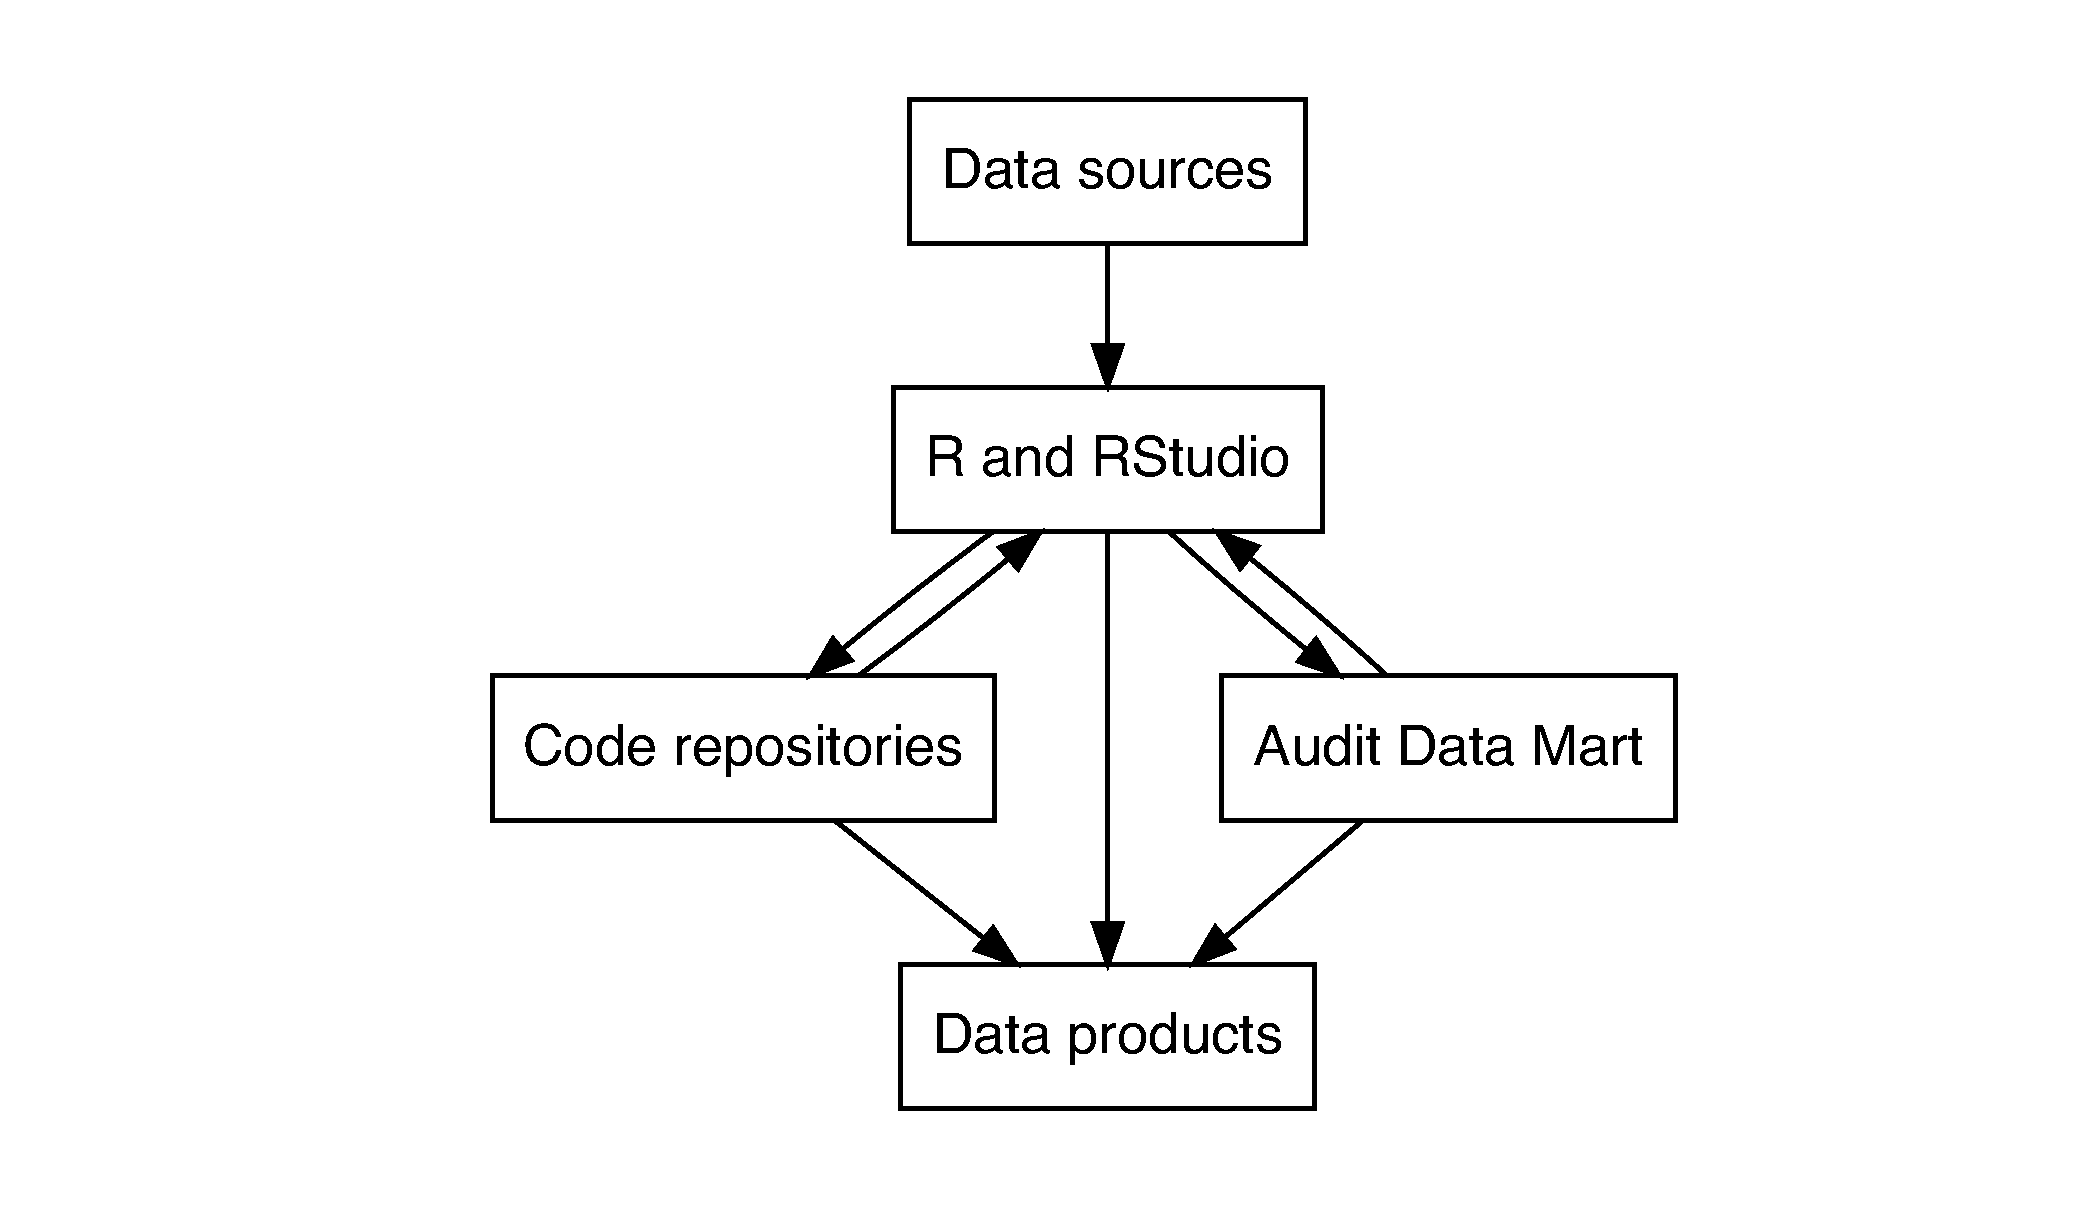
\includegraphics[width=1\linewidth]{Audit_Analytics_with-R_files/figure-latex/architecture-1} 

}

\caption{Internal Audit Data Analytics Architecture}\label{fig:architecture}
\end{figure}

The architecture and tools you select should support and amplify your team, and not be a burden to maintain. Maintenance of databases and applications can also be delegated to application support teams, so you can focus on implementing analytics and delivering data products.

Other things to consider: You should have, at a bare minimum, direct access to read-only internal databases or data warehouses. A generic service user account has its merits here when it comes to automation - tying an eventual automation to a user with password changes every 90 days will make the job feel like quarterly financial reporting.

Any software you consider should be able to talk to your company's internal applications and capabilities. Be wary of software that locks you in, as it limits your ability to integrate with your company's tools as you get more sophisticated.

\hypertarget{r-and-rstudio}{%
\section{R and RStudio}\label{r-and-rstudio}}

\href{https://www.r-project.org}{R} is a programming language with an emphasis on statistics. It is considered free software, free in the perspective that you can run, distribute, and change it as you like.

What makes R so great is the large suite of packages that are available to use to help analyze information. What doesn't exist in base R will likely have been developed by someone else: there are hundreds of packages that support data connectivity (\href{https://cran.r-project.org/web/packages/DBI/}{DBI}, \href{https://cran.r-project.org/web/packages/xlsx/}{xlsx}), day-to-day manipulation and analysis (\href{https://cran.r-project.org/web/packages/dplyr/}{dplyr}, \href{https://cran.r-project.org/web/packages/ggplot2/}{ggplot2}), and even auditing (\href{https://cran.r-project.org/web/packages/jfa/}{jfa}, \href{https://cran.r-project.org/web/packages/MUS/}{MUS}). CRAN is the central repository for all these packages that meet minimum quality standards.

As R is a language, you may want to consider an application to code in, similar to how you may write memos in Microsoft Word. \href{https://rstudio.com}{RStudio Desktop} is an integrated development environment (IDE) that has an open source version and is free to use. There are also free versions of RStudio Server, as well as commercially supported versions of its Desktop, Server, and two unique products that we will go into more later - Package Manager and Connect.

With both R and RStudio installed, you can perform the minimum requirements of your audit data analysis career: you can download data, wrangle it, visualize it, and save completed analyses. The potential is limitless though, as it enables all the other technologies to operate with it - machine learning, automation, dashboarding, and code sharing.

\hypertarget{code-repositories}{%
\section{Code repositories}\label{code-repositories}}

Here is a typical logistical challenge faced in even the smallest of audit teams. Person A will write the first version of a script to download data (V1). Person B in the team may want to use it to download data from elsewhere, so they will get an emailed script file from person B, modify it, and start to use it. Person A may make improvements to their own file, but Person B will never see the improvements. Knowledge are immediately siloed, and changes become more difficult to share between auditors.

One of the most effective ways to solve this problem is to leverage a code repository (also known as version control). While version control has several software engineering advantages, the most notable advantages for audit teams are:

\begin{itemize}
\tightlist
\item
  Centralizing domain knowledge and sharing code,
\item
  Tracking and tracing changes to code throughout time (including who, what was changed, and when), and
\item
  Ability to test with an isolated code set before rolling out to production.
\end{itemize}

Code versioning technologies resonate closely with IT General Controls and even the COBIT framework.

\hypertarget{git}{%
\subsection{Git}\label{git}}

\href{https://git-scm.com}{git} is a type of version control. Another free, open source software, and the basic usage of the tool is accessible.

The basics of git are:

\begin{itemize}
\tightlist
\item
  Pull code from the remote server to the local computer.
\item
  Write and save code on your local computer.
\item
  Commit code on your local computer.
\item
  Push code from your local computer to the remote server.
\end{itemize}

While this is a superficial example of how to use git, it is enough to get the most basic of audit teams started. The git hole can go very deep, so if things don't go according to plan, just remember that you can always \href{https://xkcd.com/1597/}{make a new folder and start fresh}.

Several different server technologies support git - \href{https://github.com}{github}, \href{https://azure.microsoft.com/en-us/services/devops/repos/}{Azure Repos} within Azure DevOps, \href{https://gitlab.com}{gitlab} are all willing to host your code. If you're using these to hold proprietary or sensitive code, it would be wise to get your company's support and pay for the ability to have a private repository that only your team can see.

\hypertarget{packages}{%
\subsection{Packages}\label{packages}}

As you write more code and templates, you will eventually want to share these new techniques with others on your team. Packages put your best practices together, including templates, functions to solve common problems, and templates for common workflows. In short: packages contain tasks help you do your job, and save you time.

Packages go beyond the tangible and provide several qualitative benefits as well. They standardize your team's workflow, create consistency and readability standards, and get your team to speak a single language. It creates a cohesive foundation where anyone on the team can contribute, and a library for those who wish to learn more.

However, you do not need to force your team to copy-and-paste a folder or even a Word document from a template folder. The most elegant way to distribute your code is via packages. These packages can be hosted on a code repository, enabling your team to download best practices with a simple line of code. The packages can also be hosted privately, so only your company or team can access them.

The best part? You can give your package a creative name that represents the culture of your internal audit team or organization. Just don't call it auditR.

\hypertarget{data-products}{%
\section{Data Products}\label{data-products}}

All auditors face this problem at one point or another. An audit finding doesn't matter until someone takes accountability for it. And if an audit finding is too vague, or does not have the buy-in from the right stakeholders, it is as good as unsolicited advice.

The data analysis you deliver are exposed to the same requirements. Not only do they need to be accurate, but they also need to be accessible, relevant, and delivered at the right time. If there are too many barriers for entry or usage, someone will revert back to their old processes and methods. Here is a sobering thought: when was the last time you made a beautiful visualization for someone, only to be asked for the detailed Excel worksheet afterwards? Or instead of an automated report that users can self-serve, someone asks for an email instead?

Data products are deliverable that enhance your customer's ability to gather, process and analyze information. They facilitate decision making and are integrated into their processes. They should be designed thoughtfully and simply, masking the complexity underneath. In short, they should make your co-auditors feel like rockstars. The reports you write and code you develop should strive for the goal of being accessible by your team, on-time and on-demand.

\hypertarget{galvanize-highbond}{%
\subsection{Galvanize Highbond}\label{galvanize-highbond}}

\href{https://www.wegalvanize.com}{Galvanize}, the parent company of ACL Analytics and one of the most popular companies in the audit software industry, invested significant efforts into their cloud-based working paper solution, Highbond. One of their modules, Highbond Results, is fantastic for audit exception and remediation workflow.

The idea with an audit exception workflow is that audit testing will identify an actionable transaction or outcome. This may be an exception within a process, a control requiring execution, or even a request for additional information or clarification. Once a process has been designed, Highbond Results will allow you to focus on the users who should action the workflow and the rules for setting up triggers.

While Galvanize is a separate, third-party product that is not R-related, it does integrate with R through its API. The API enables you to upload findings and results directly into a Results set, allowing you to create the workflows on the website. The API also enables access to its Projects data that your audit team may already use to document audits, offering advantages to audit teams ambitious enough to design their workpaper environments effectively.

Highbond Results also provides capabilities to do no-code based visualizations hosted on the web. Once set up, they offer a stable method of delivering storyboards and visualizations.

Galvanize cloud-based tools are fully hosted, meaning audit teams pay for high availability and security maintained by a professional team. Galvanize supports the \href{https://www.wegalvanize.com/trust/}{security}, design and coding for hosting a tool online, allowing you to focus on designing workflows for your internal customers.

\hypertarget{rstudio-connect}{%
\subsection{RStudio Connect}\label{rstudio-connect}}

RStudio PBC, which became a Certified B Corporation in 2020, offers the \href{https://rstudio.com/products/connect/}{RStudio Connect} solution that allows R deliverable to be hosted online. These include:

\begin{itemize}
\tightlist
\item
  \href{https://rmarkdown.rstudio.com}{RMarkdown} notebooks, which are fully self-contained analytics. These notebooks perform full analyses from start to finish, including downloading data, wrangling, analysis and data visualization.
\item
  These notebooks can also act at Extract, Transform, and Load processes. These notebooks have the advantage of being automatically scheduled, with rules that can notify stakeholders if need be. The loading component can be any destination - most popular is the audit data mart, or into other web applications via API connectivity (example: Galvanize Highbond Results).
\item
  The hosting of \href{https://shiny.rstudio.com}{Shiny} apps, which are interactive web applications, offer a way to analyze and present information in an intelligent, slick manner. The analysis performed in R can be factored into a Shiny app, which can be hooked directly into your data.
\end{itemize}

For audit teams who have expertise in programming, RStudio Connect offers some of the best capabilities for pushing out visualizations and analysis to your teams and internal stakeholders.

RStudio server software will require talent to stand-up and maintain, and should be considered in an environment where automation and internal hosting of data products will bring advantages to an internal audit team.

\hypertarget{rstudio-package-manager}{%
\subsection{RStudio Package Manager}\label{rstudio-package-manager}}

RStudio Package Manager offers the capability to

\hypertarget{data-sources}{%
\section{Data sources}\label{data-sources}}

\hypertarget{databases}{%
\subsection{Databases}\label{databases}}

\hypertarget{external-sources}{%
\subsection{External sources}\label{external-sources}}

\hypertarget{setup}{%
\chapter{Setup}\label{setup}}

\hypertarget{rstudio}{%
\section{RStudio}\label{rstudio}}

\hypertarget{github}{%
\section{Github}\label{github}}

\hypertarget{audit-analytics}{%
\chapter{Audit analytics}\label{audit-analytics}}

\hypertarget{import-data}{%
\section{Import data}\label{import-data}}

\hypertarget{explore}{%
\section{Explore}\label{explore}}

\hypertarget{manipulate}{%
\section{Manipulate}\label{manipulate}}

\hypertarget{report}{%
\section{Report}\label{report}}

\hypertarget{applied-audit-analytics}{%
\chapter{Applied audit analytics}\label{applied-audit-analytics}}

\hypertarget{package-creation}{%
\section{Package creation}\label{package-creation}}

\hypertarget{continious-monitoring}{%
\section{Continious Monitoring}\label{continious-monitoring}}

\hypertarget{controls-automation}{%
\section{Controls automation}\label{controls-automation}}

\hypertarget{audit-data-mart}{%
\section{Audit Data Mart}\label{audit-data-mart}}

\hypertarget{all-in-one-toolkits}{%
\section{All-in-one toolkits}\label{all-in-one-toolkits}}

\hypertarget{other-practices-to-follow}{%
\chapter{Other practices to follow}\label{other-practices-to-follow}}

\hypertarget{passwords}{%
\section{Passwords}\label{passwords}}

\hypertarget{section}{%
\section{}\label{section}}

\hypertarget{audit-data-products}{%
\chapter{Audit data products}\label{audit-data-products}}

  \bibliography{book.bib,packages.bib}

\end{document}
